\begin{figure}[h]
  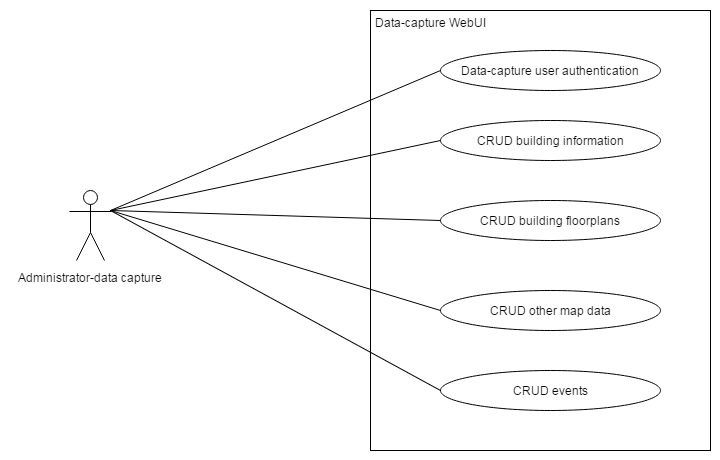
\includegraphics[width=\textwidth]{diagrams/Specific_Requirements/data_capture_WebUI.png}
\end{figure}

The data-capture adds the system's metadata such as building location , history ,campus events etc. Since the system will provide indoor navigation the metadata indoors will not be entirely visible on the external map hence upon entrance of a building the map needs to change to display a buildings internal map.

\FuncReq
{Data-capture user authentication}
{The usual things are required for authentication}
{Trivial}
{Trivial}

\FuncReq
{CRUD building information}
{CRUD of building information. This includes building names, positions and historical trivia.}
{Trivial}
{Trivial}

\FuncReq
{CRUD building floorplans}
{CRUD of building floorplans include location of rooms and disability ramps as well as conventional stairs.}
{Trivial}
{Trivial}

\FuncReq
{CRUD other map data}
{This includes routes, walkways, roads, entrances and other landmarks such as artwork.}
{Trivial}
{Trivial}
 
\FuncReq{CRUD events}
{Trivial}
{Trivial}
{Trivial}
